\documentclass[11pt]{article}

\usepackage[margin=1in]{geometry}
\usepackage{times}
\usepackage{graphicx}
\usepackage{booktabs}
\usepackage{amsmath}
\usepackage{hyperref}
\usepackage{microtype}
\usepackage{xcolor}

\title{Characterizing Single-GPU Decoder-Only Transformer Inference:\\
Precision, Compilation, Batching, and Sequence Length on an RTX 5070}
\author{Ben Karlsberg}
\date{}

\begin{document}
\maketitle

\begin{abstract}
We present a controlled single-GPU study of decoder-only transformer inference using a small open causal language model.
On an NVIDIA GeForce RTX~5070, we measure synchronized end-to-end \texttt{generate()} latency and tokens-per-second across a 32-cell matrix spanning data type (FP16, BF16), batch size (1, 4), prompt length (64, 256), generation length (32, 128), and execution mode (eager vs.\ \texttt{torch.compile}).
All cells completed without out-of-memory failures.
BF16 reduced end-to-end latency relative to FP16 in every paired comparison (median BF16/FP16 latency ratio $0.90$).
Increasing batch size from 1 to 4 raised throughput by roughly $4\times$ while keeping wall-clock latency in a similar range.
Generation length dominated end-to-end time, while tokens-per-second stayed comparatively flat, consistent with decode-bound behavior under this harness.
\texttt{torch.compile} yielded a median eager/compile latency ratio of $1.02$ (range $0.92$--$1.22$), indicating little systematic gain for this model and measurement window.
We release the harness, configurations, and aggregated results to support reproduction.
\end{abstract}

\section{Introduction}
Autoregressive transformer inference~\cite{vaswani2017attention} is commonly deployed with mixed precision, compiler stacks, and request batching.
Practitioners must choose among these options without assuming that every optimization helps every workload.
This paper reports a small, reproducible characterization on one consumer GPU using the open-source \texttt{goti} harness accompanying this work.
Our goal is empirical clarity on a fixed model and hardware point---not a claim of state-of-the-art serving performance.

\section{Method}
\subsection{Software stack}
Experiments use PyTorch~\cite{paszke2019pytorch} with CUDA~12.8 bindings (\texttt{torch 2.11.0+cu128}), Hugging Face Transformers for model loading, and scaled-dot-product attention via PyTorch SDPA backends.
The workload is greedy \texttt{model.generate()} with KV caching enabled.
Synthetic token ids form prompts so logging of decoded text cannot contaminate timed regions.

\subsection{Metrics and timing protocol}
For each configuration we run a warmup phase followed by measured iterations.
Each iteration records GPU-synchronized end-to-end latency of \texttt{generate()}, peak CUDA memory allocated, and tokens-per-second derived from generated token count and wall time.
We report distributional summaries (mean, selected percentiles) rather than a single timing.
Cold-start model load is outside the measured loop; \texttt{torch.compile} configurations still include steady measured iterations after warmup, but compilation cost can affect short windows and is treated as part of the system under test.

\subsection{Experimental matrix}
Model: \texttt{HuggingFaceTB/SmolLM-135M}.
Factors: dtype $\in\{\mathrm{fp16},\mathrm{bf16}\}$, batch size $\in\{1,4\}$, prompt length $\in\{64,256\}$, max new tokens $\in\{32,128\}$, compile $\in\{\mathrm{false},\mathrm{true}\}$.
This yields 32 cells.
Hardware: NVIDIA GeForce RTX~5070 (driver 610.62, $\approx$12\,GB), host BensPC, Windows~10.

\section{Results}
All 32 cells completed with no OOM events.
The lowest mean end-to-end latency was $586$\,ms (BF16, batch~4, prompt~256, gen~32, compile enabled; $\approx$218 tok/s).
The highest was $2855$\,ms (FP16, batch~4, prompt~64, gen~128, eager; $\approx$180 tok/s).

\subsection{Precision}
Figure~\ref{fig:dtype} compares FP16 and BF16 latency for every matched non-dtype factor.
BF16 was faster in all 16 pairs.
The median BF16/FP16 latency ratio was $0.895$ (mean $0.890$).

\begin{figure}[t]
\centering
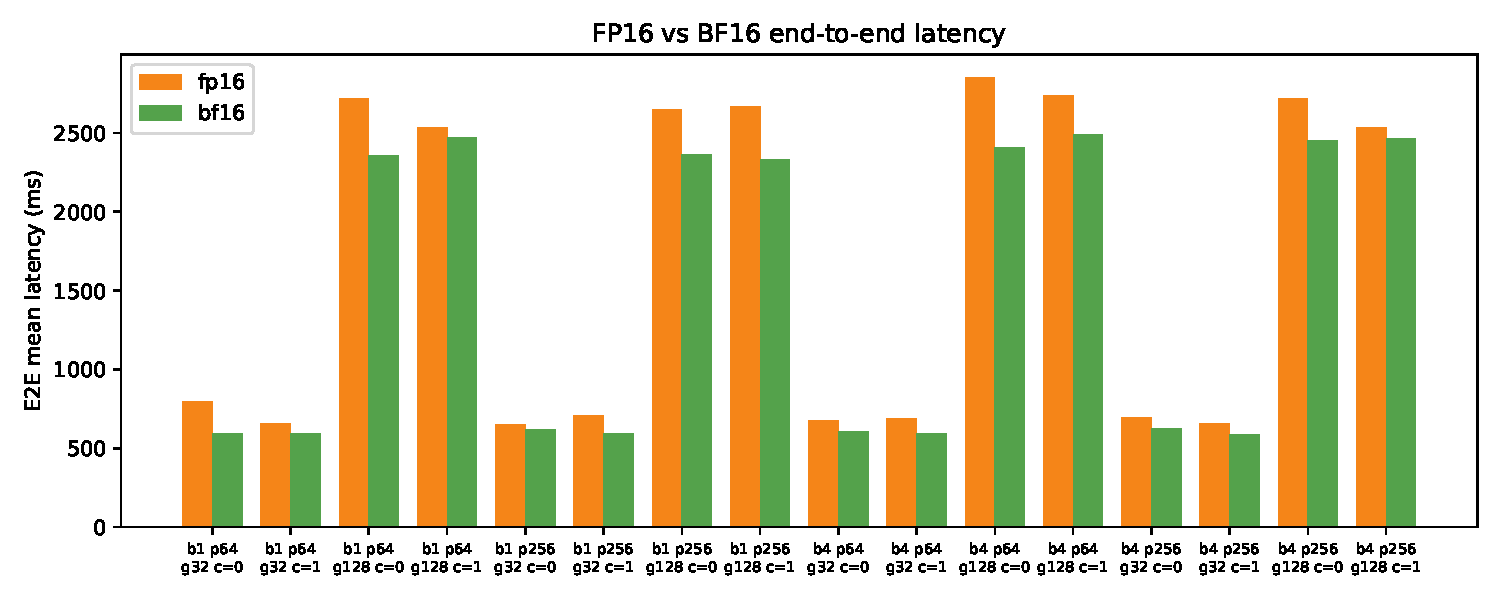
\includegraphics[width=\linewidth]{figs/dtype_latency.pdf}
\caption{End-to-end mean latency for FP16 vs.\ BF16 across matched matrix cells.}
\label{fig:dtype}
\end{figure}

\subsection{Batching and throughput}
Figure~\ref{fig:batch} shows tokens-per-second versus batch size for FP16 eager runs.
Moving from batch~1 to batch~4 increased throughput from roughly $40$--$50$ tok/s to roughly $180$--$210$ tok/s.
End-to-end latency did not scale linearly with batch size, illustrating the usual serving tradeoff: batching amortizes work across requests more than it reduces single-request latency.

\begin{figure}[t]
\centering
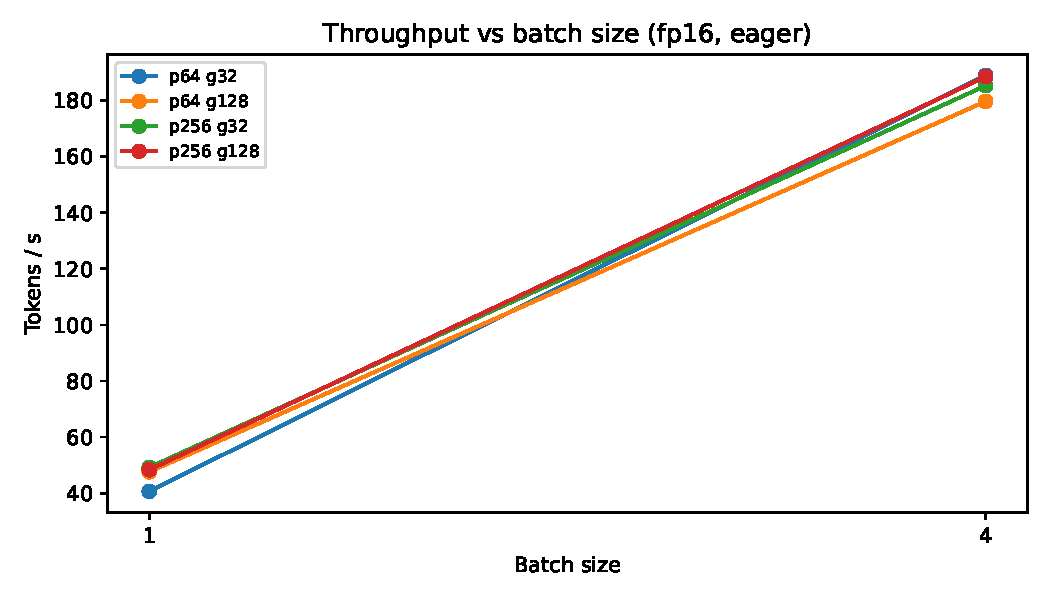
\includegraphics[width=0.85\linewidth]{figs/batch_throughput.pdf}
\caption{Throughput versus batch size (FP16, eager).}
\label{fig:batch}
\end{figure}

\subsection{Generation length}
Figure~\ref{fig:gen} plots latency against generated token count for BF16 eager batch~1.
Increasing generation length from 32 to 128 raised end-to-end latency by roughly $4\times$, while tokens-per-second remained near $50$--$55$ tok/s.
Under this harness, wall-clock time tracks decode length more strongly than the modest prompt-length change ($64$ vs.\ $256$).

\begin{figure}[t]
\centering
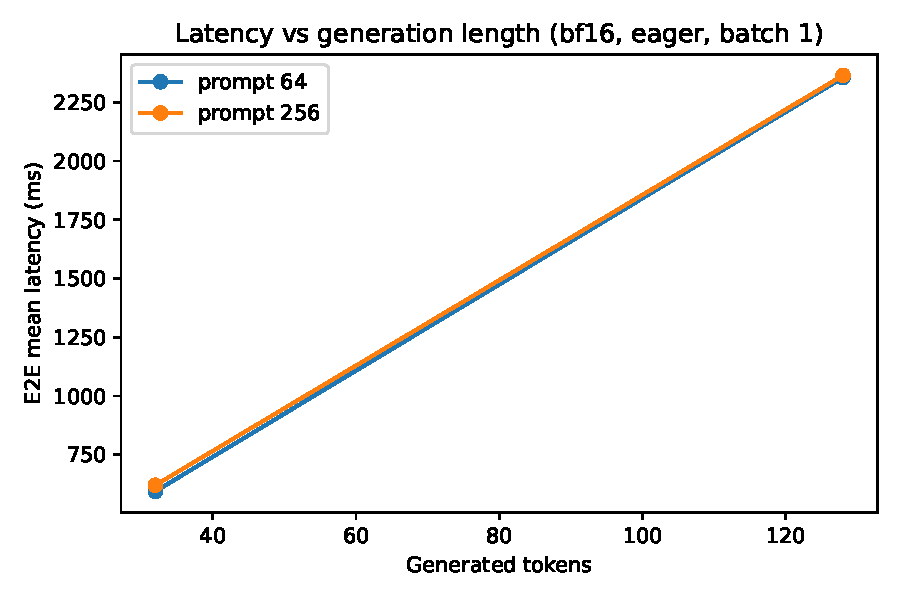
\includegraphics[width=0.75\linewidth]{figs/gen_latency.pdf}
\caption{Latency versus generation length (BF16, eager, batch 1).}
\label{fig:gen}
\end{figure}

\subsection{Compilation}
Figure~\ref{fig:compile} reports eager/compile latency ratios.
The median ratio was $1.015$ (mean $1.027$), ranging from $0.921$ to $1.218$.
Thus \texttt{torch.compile} was approximately neutral on average for this model and measurement protocol, with occasional gains or regressions depending on the cell.

\begin{figure}[t]
\centering
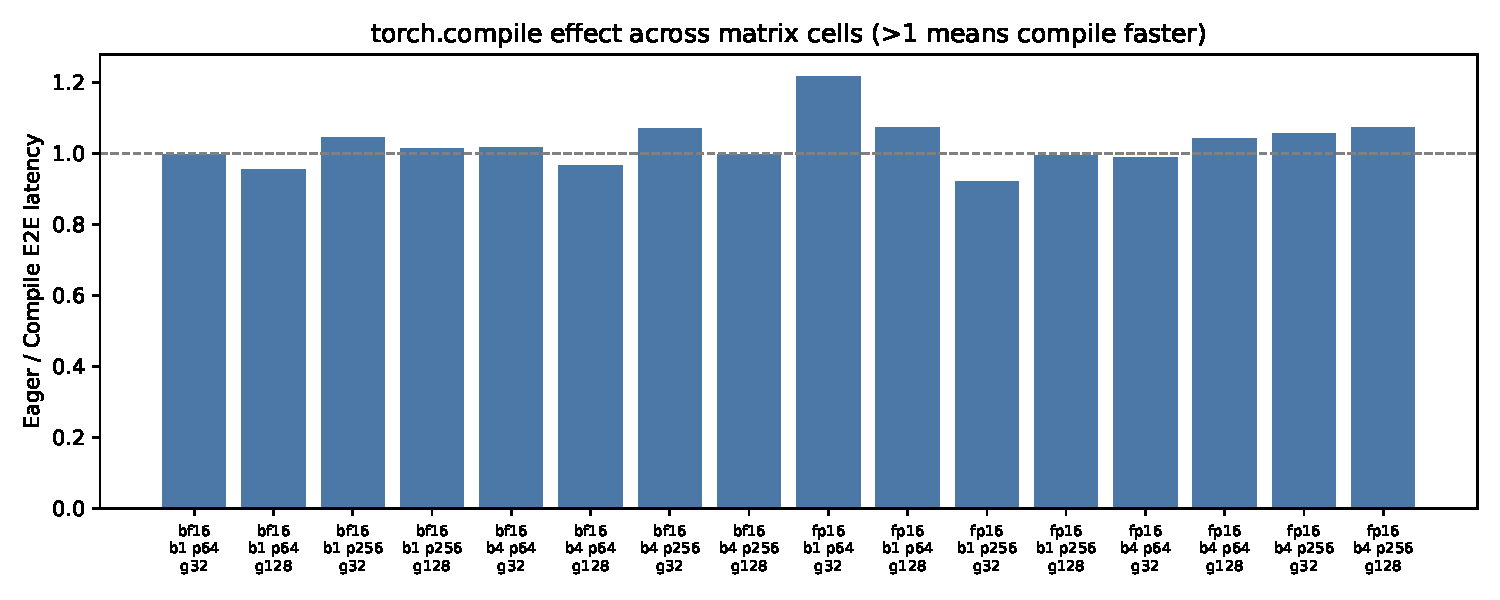
\includegraphics[width=\linewidth]{figs/compile_speedup.pdf}
\caption{Eager/compile end-to-end latency ratios ($>1$ means compile is faster).}
\label{fig:compile}
\end{figure}

\section{Discussion and limitations}
These measurements characterize one GPU, one small model, and an end-to-end \texttt{generate()} timer.
They do not isolate time-to-first-token or inter-token latency, do not evaluate weight quantization or continuous batching under load, and do not claim optimality of any backend.
Within that scope, four conclusions are stable in the data: BF16 reduced latency vs.\ FP16; batching primarily improved throughput; generation length dominated wall time; and \texttt{torch.compile} did not provide a consistent speedup.

\section{Conclusion}
We measured a full 32-cell inference matrix on an RTX~5070 using a reproducible harness.
The results emphasize workload- and precision-dependent behavior and caution against assuming that compilation alone improves short, small-model inference runs.
Code and aggregated artifacts are available in the accompanying repository.

\bibliographystyle{plain}
\begin{thebibliography}{9}

\bibitem{vaswani2017attention}
A.~Vaswani, N.~Shazeer, N.~Parmar, J.~Uszkoreit, L.~Jones, A.~N. Gomez, \L.~Kaiser, and I.~Polosukhin.
\newblock Attention is all you need.
\newblock In {\em Advances in Neural Information Processing Systems}, volume~30, pages 5998--6008, 2017.

\bibitem{paszke2019pytorch}
A.~Paszke, S.~Gross, F.~Massa, A.~Lerer, J.~Bradbury, G.~Chanan, T.~Killeen, Z.~Lin, N.~Gimelshein, L.~Antiga, A.~Desmaison, A.~Kopf, E.~Yang, Z.~DeVito, M.~Raison, A.~Tejani, S.~Chilamkurthy, B.~Steiner, L.~Fang, J.~Bai, and S.~Chintala.
\newblock PyTorch: An imperative style, high-performance deep learning library.
\newblock In {\em Advances in Neural Information Processing Systems}, volume~32, pages 8024--8035, 2019.

\end{thebibliography}

\end{document}
